\documentclass{beamer}
\usepackage{beamerthemeshadow}
\usepackage[english]{babel}

\begin{document}
\title{Modeling Variable Throughput Channels with Stochastic ODEs}  
\author{D. Masi, P. Pegus II , J. M. Wong}
\date{\today} 

\frame{\titlepage} 

\frame{\frametitle{Outline}\tableofcontents} 

\section{Introduction} {
	\frame{\frametitle{Introduction} {
		\begin{figure}[H]
		\centering
		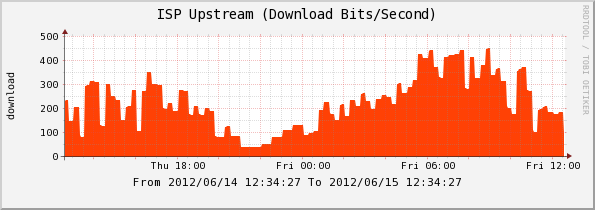
\includegraphics[scale=.40]{Images/throughput.png}
		\end{figure}
		Stochastic differential equations are often used to model the nondeterministic behavior of network channels in computer science.
		}
	}
	\subsection{Networking Basics} {
		\frame{\frametitle{Networking Basics} {
			A \textbf{Channel} is the medium through which a message propagates from sender to receiver.
			\begin{figure}[H]
			\centering
			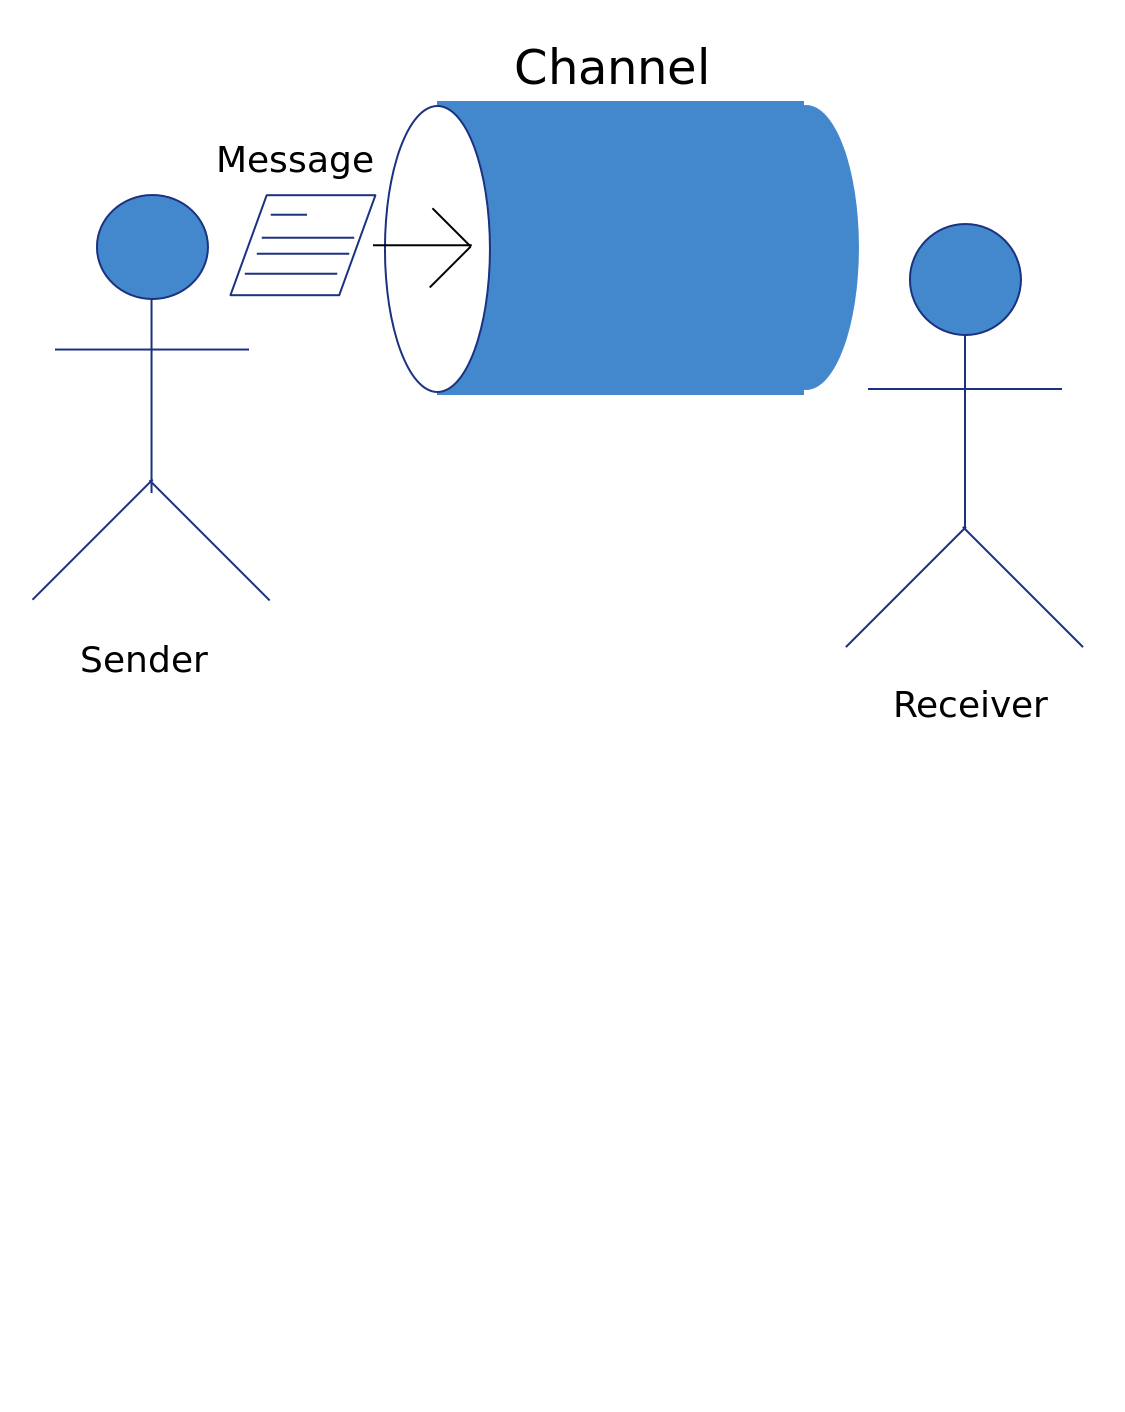
\includegraphics[scale=.20]{Images/network_components.png}
			\end{figure}
			}
		}
	}
	\subsection{Channel Characteristics} {
		\frame{\frametitle{Channel Characteristics} {
			\begin{figure}[H]
			\centering
			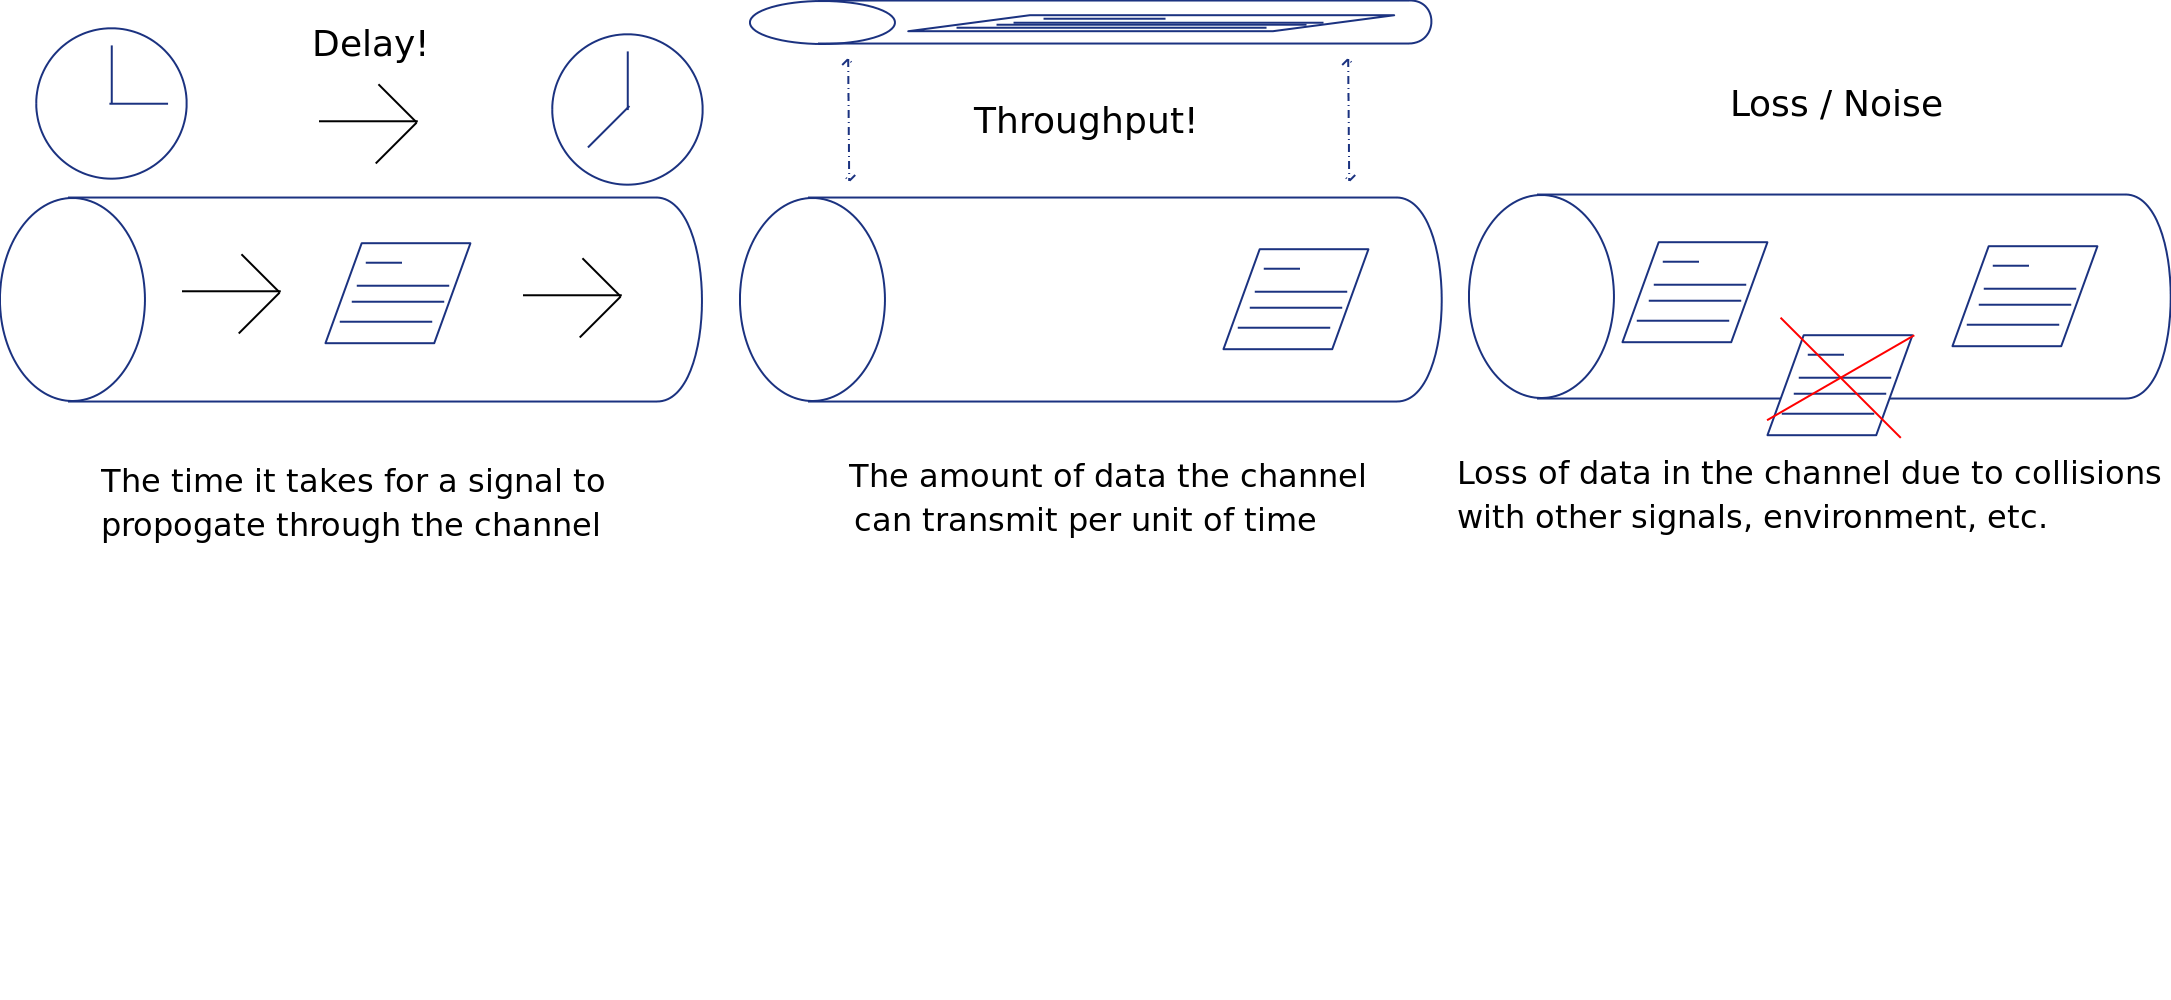
\includegraphics[scale=.15]{Images/channel_characteristics.png}
			\end{figure}
			}
		}
	}
}

\section{Image Compression} {
	\frame{\frametitle{Image Compression} {
		\begin{figure}[H]
		\centering
		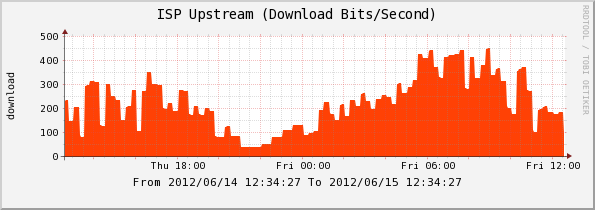
\includegraphics[scale=.40]{Images/throughput.png}
		\end{figure}
		Stochastic differential equations are often used to model the nondeterministic behavior of network channels in computer science.
		}
	}
	\subsection{Compression Using Low Pass} {
		\frame{\frametitle{Compression Using Low Pass} {
			A \textbf{Channel} is the medium through which a message propagates from sender to receiver.
			\begin{figure}[H]
			\centering
			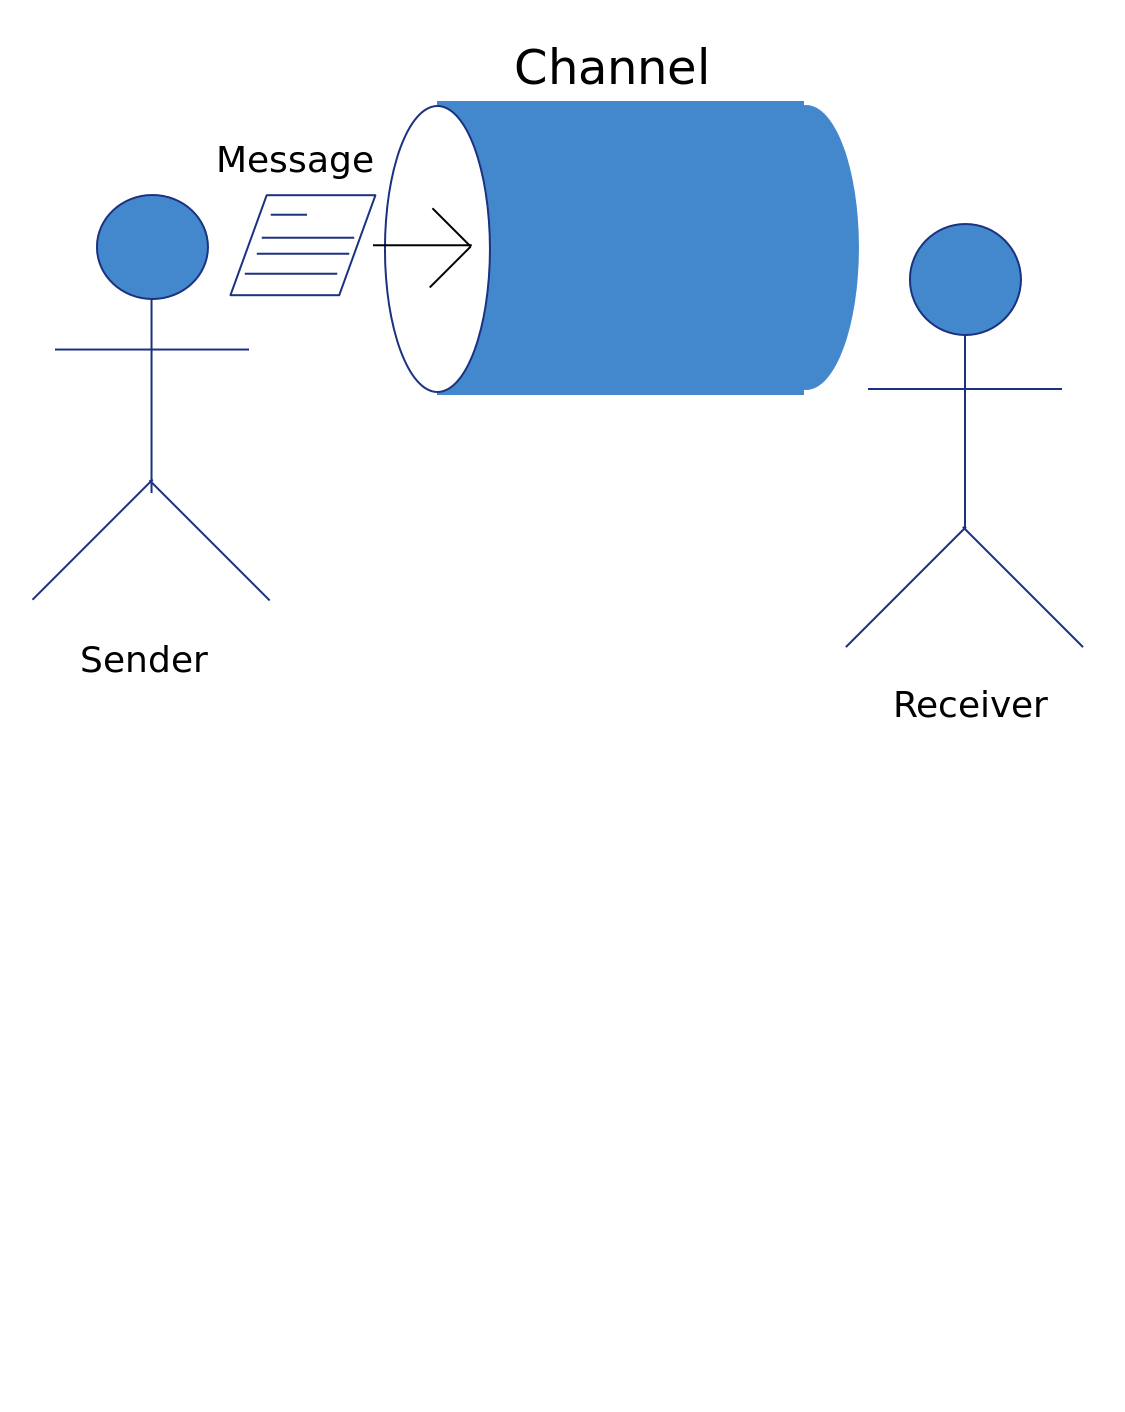
\includegraphics[scale=.20]{Images/network_components.png}
			\end{figure}
			}
		}
	}
	\subsection{Compression Using Average} {
		\frame{\frametitle{Compression Using Average} {
			A \textbf{Channel} is the medium through which a message propagates from sender to receiver.
			\begin{figure}[H]
			\centering
			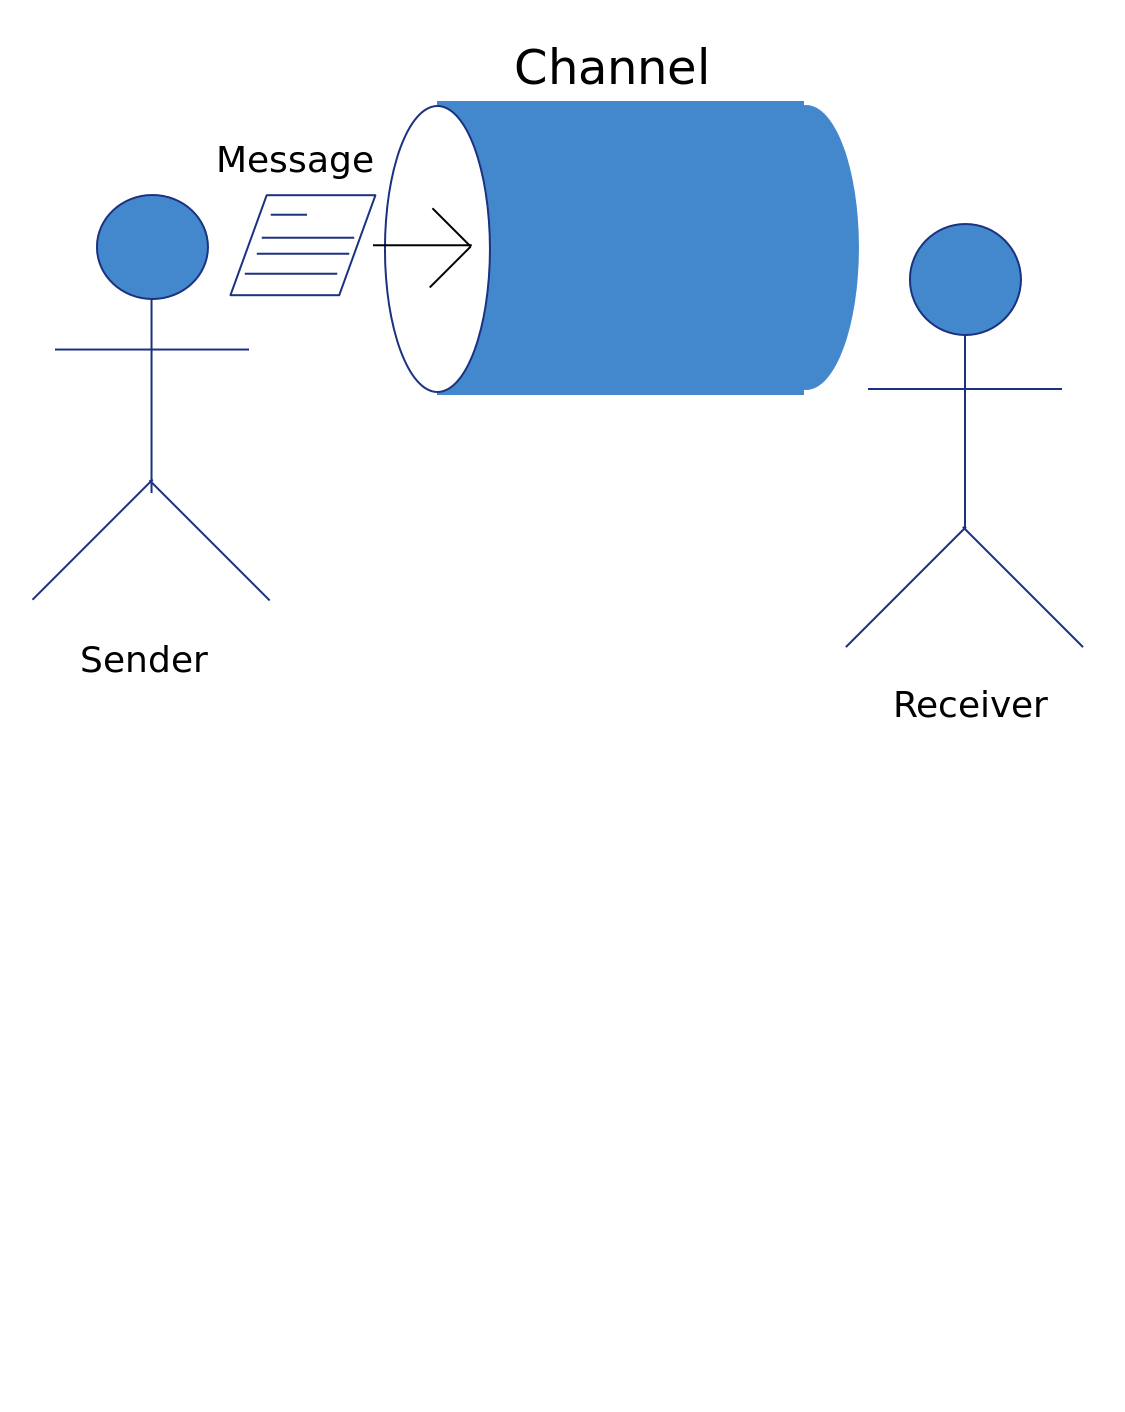
\includegraphics[scale=.20]{Images/network_components.png}
			\end{figure}
			}
		}
	}
}

\section{Implementation}{
\subsection{Euler-Marauyama Method} {
		\frame{\frametitle{Euler-Marauyama Method} {
			We approximate the solution by assigning y-values $w_0 < w_1 < w_2 < \cdots < w_n$ at discretized $t$, given the SDE IVP
			\begin{equation}
				dy(t) = f(y,t)dt+g(t,y)dB_t
			\end{equation}
			\begin{equation}
				y(a) = y_a
			\end{equation}
			\begin{figure}[H]
			\centering
			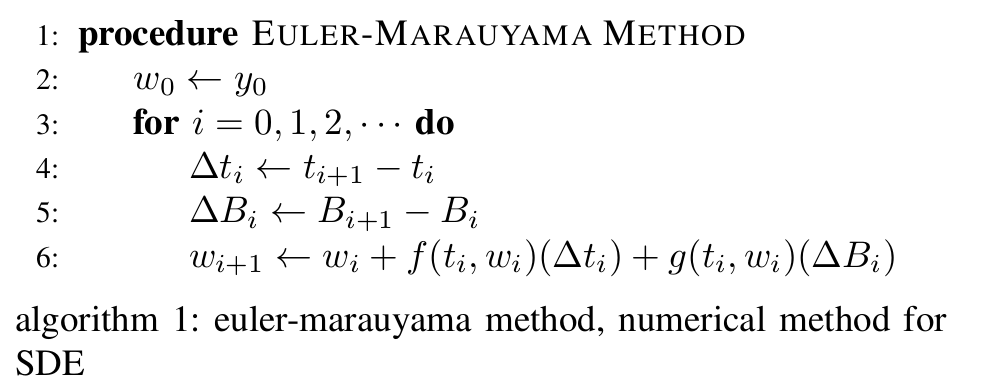
\includegraphics[scale=.3]{Images/euler.png}
			\end{figure}
			}
		}
	}


}
\section{Demonstration}{
	\frame{\frametitle{Demonstration} {
		\begin{figure}[H]
		\centering
		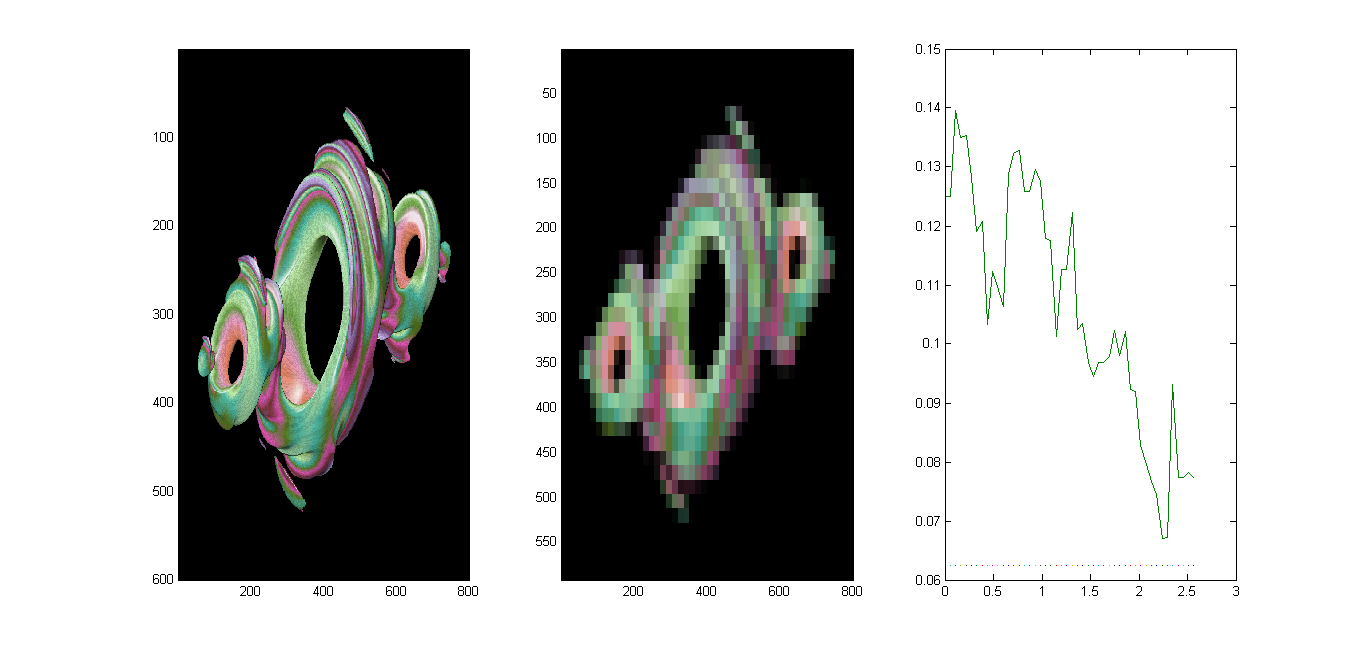
\includegraphics[scale=.30]{Images/img.png}
		\end{figure}
}

}

}

\end{document}
\section{Demonstration}{
	\frame{\frametitle{Demonstration} {
		\begin{figure}[H]
		\centering
		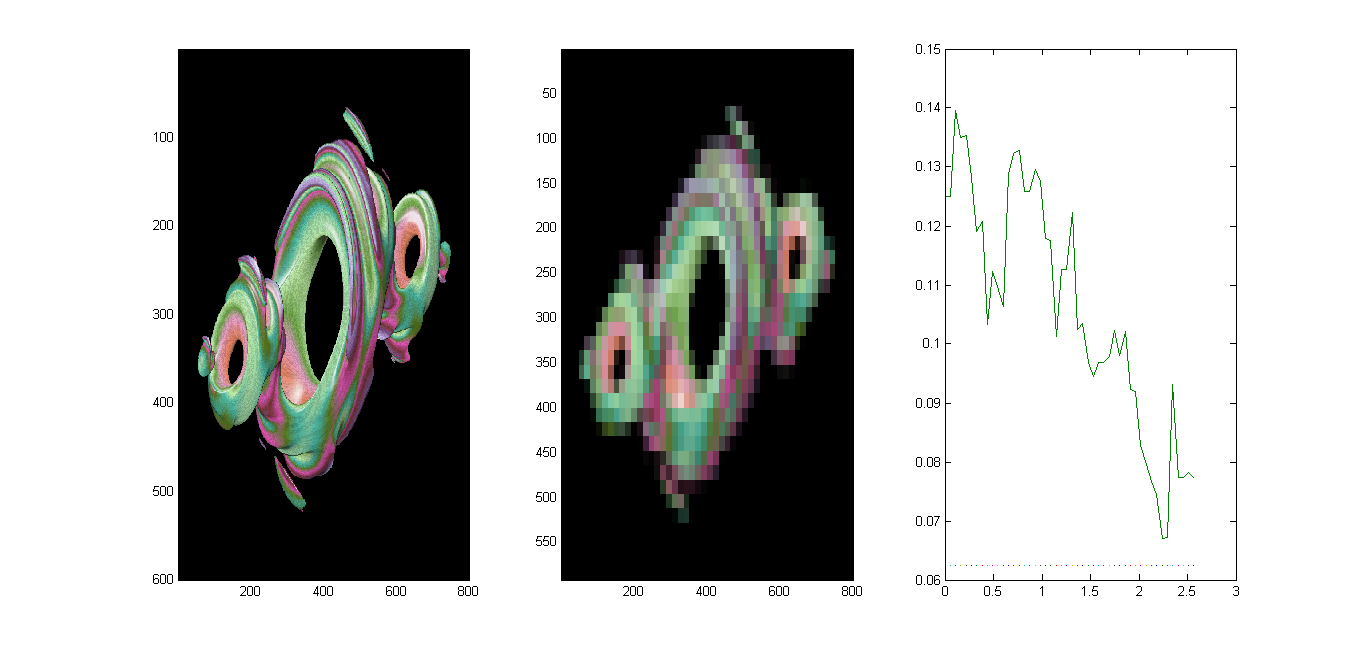
\includegraphics[scale=.30]{Images/img.png}
		\end{figure}
}

}

}

\end{document}

